This chapter presents an overview of the different steps taken to fully implement a functional system by exploring the entire system pipeline. The chapter begins with the first stage of pipeline, the offline colour-based feature extraction phase, where histograms are extracted and averaged into compact signatures for each database video before being saved in files. Next, the second stage of the pipeline is covered, the online retrieval phase, explaining how the query video is matched to one of the database videos using the compact histograms previously generated. Finally, the final optional stage of the pipeline is explored, the database pre-processing phase, explaining how videos can be segmented into smaller videos. These three phases of the pipeline culminate with the flowchart diagram representing the entire system. Figures, mathematical formulas and code snippets are used to assist with examples and clearer visualisations. To round off the chapter, the code structure of the project is covered, along with a few words on testing. 

% TODO: mention argument parsing somewhere

%%%%%%%%%%%%%%%%%%%%%%%%%%%%%%%%%%%%%%%%%%%%%%%%%%%%%%%%%%%%%%%%%%%%
%%%%%%%%%%%%%%%%%%%%%%%%%%%%%%%%%%%%%%%%%%%%%%%%%%%%%%%%%%%%%%%%%%%%
%%%%%%%%%%%%%%%%%%%%%%%%%%%%%%%%%%%%%%%%%%%%%%%%%%%%%%%%%%%%%%%%%%%%

\section{Offline Colour-Based Feature Extraction}
\label{sec:implementation-offline-colour-based-feature-extraction}

This section details the different steps that go towards extracting colour features from the database videos to generate histograms and creating the compact signature used to represent each video. The first step consists in establishing a selection of frames to process, followed by generating histograms for each of those selected frames. Once the histograms are generated, they are averaged into a single histogram before being normalised and stored into a plain text file. Figure \ref{fig:implementation-rgb_average_histogram_pipeline} demonstrates a visual example of inner pipeline of this phase with RGB histograms only. This phase is repeated for greyscale and HSV histograms as well).\\

\begin{figure}[h] 
\centerline{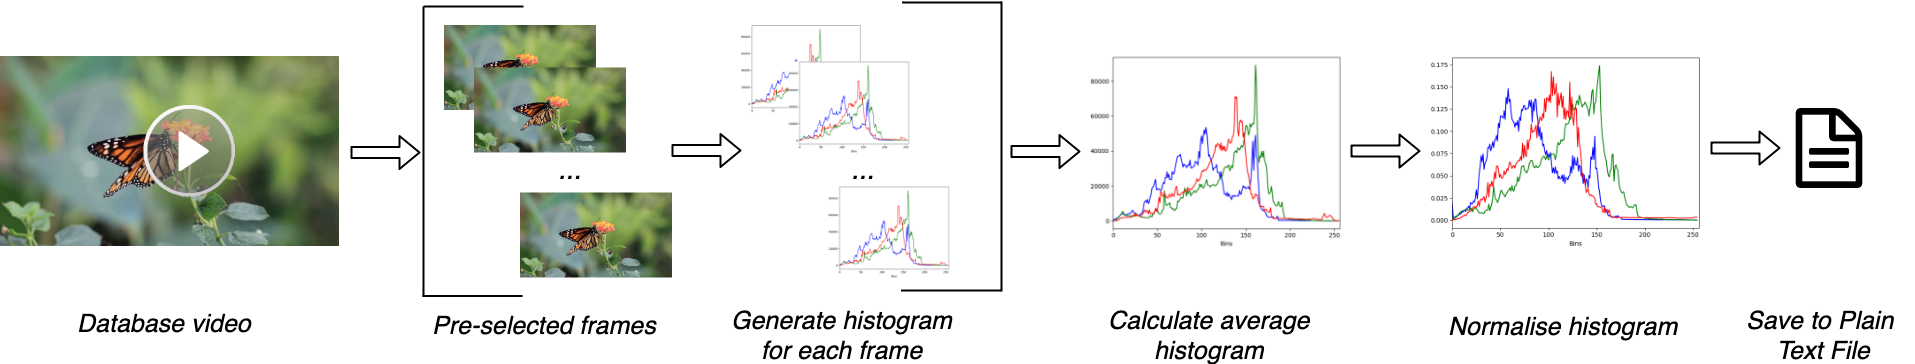
\includegraphics[width=1.2\textwidth,center]{figures/implementation/rgb_average_histogram_pipeline.png}}
\caption{\label{fig:implementation-rgb_average_histogram_pipeline}Visualisation of the pipeline of the offline colour-based feature extraction phase with RGB histograms only.}
\end{figure}

This phase has to be repeated for every video in the database. For consistency throughout the various examples that are illustrated in this section, the \textit{butterfly} video is used to provide examples of the multiple offline colour-based feature extraction steps.

%%%%%%%%%%%%%%%%%%%%%%%%%%%%%%%%%%%%%%%%%%%%%%%%%%%%%%%%%%%%%%%%%%%%

\subsection{Histogram Generation}

As described in Section \ref{sec:color-based-features}, a histogram represents the distribution of the pixels in a single frame. Different types of histograms can be generated based on the colour model used. This section covers how three types of histograms are constructed based on the colour model used, starting with greyscale histograms, followed by RGB histograms and ending with HSV histograms.

%%%%%%%%%%%%%%%%%%%%%%%%%%

\subsubsection{Greyscale Histogram}
\label{sec:implementation-greyscale-histogram}

The first type of histogram that is generated is the greyscale histogram, also known as an intensity-based histogram. This type of histogram is used with frames that are first converted to a black \& white colour space (see Figure \ref{fig:rgb_to_greyscale}), and thus has a single channel rather than the three traditional RGB channels found in colour images. The conversion is done using OpenCV's \textit{cv2.cvtColor()} function along with the \textit{cv2.COLOR\_BGR2GRAY} attribute: 
\mint[fontsize=\footnotesize]{python}|grey_frame = cv2.cvtColor(frame, cv2.COLOR_BGR2GRAY)|

\begin{figure}[h] 
\centerline{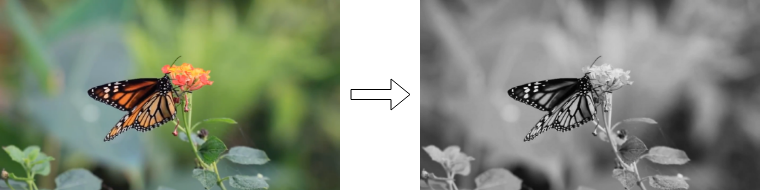
\includegraphics[width=\textwidth]{figures/implementation/rgb_to_greyscale.png}}
\caption{\label{fig:rgb_to_greyscale}Conversion of a frame from the RGB colour space to greyscale (black \& white).}
\end{figure}

Because the video frames are 8-bit images, the spectrum of the potential pixel values ranges between 256 possible values\footnote{$2^8=256$}. As a result, the histogram has 256 different bins from 0 to 255 to represent all the potential values that each pixel can take. The histogram itself is portrayed by Equation \ref{eq:grey-histogram}, where $g\in [0, 255]$ and $N_g$ represents the number of pixels that have an intensity equal to $g$. For example, $H(30)$ represents the number of pixels in the image with an intensity value of 30.
\begin{equation}
\label{eq:grey-histogram}
    H(g)=N_g
\end{equation}

The implementation of the greyscale histogram generation in the system is carried out through OpenCV's \textit{calcHist()} method, with the result portrayed in Figure \ref{fig:implementation-greyscale_not_normalised}. The grey frame is passed to the function, along with the number of channels to use, which is a single one in this case ($[0]$), an empty mask $None$ since the histogram is being calculated for the full frame, the number of bins $[256]$, and the range of values $[0, 256]$:

\mint[fontsize=\footnotesize]{python}|histogram = cv2.calcHist([grey_frame], [0], None, [256], [0,256])|

\begin{figure}[h] 
\centerline{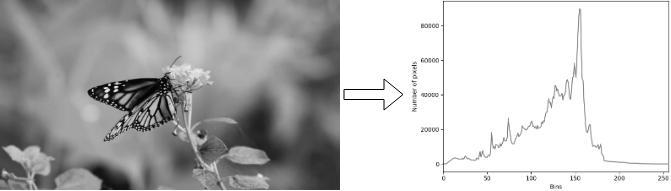
\includegraphics[width=\textwidth]{figures/implementation/greyscale_not_normalised.png}}
\caption{\label{fig:implementation-greyscale_not_normalised}The generated greyscale histogram (not normalised).}
\end{figure}

These greyscale histograms are generated for multiple frames of the video, but not all the frames as this would be highly inefficient, as explained in Section \ref{sec:litsurvey-challenges-temporality}. Indeed, rather than generating a histogram for each frame, which would be extremely inefficient and waste of computations, a selection of frames can be made in advance, which is then used for the histogram generation. Ideally, the frames extracted from the shot boundary detection algorithm later described in Section \ref{sec:database-pre-processing} are used. However, because the scope of the duration of the videos used is between 7 and 14 seconds and they are only made of a single shot, the shot boundary detection algorithm would only extract one frame from the videos. Therefore, for the purpose of building a realistic system, one frame is extracted every second to build up the selection of frames, using the \textit{\_get\_frames\_to\_process()} function from Appendix \ref{sec:code-listings-get-frames-to-process}. For example, with the butterfly video that contains 301 frames and has a frame rate of 30 frames per second, 11 frames are selected to generate a greyscale histogram (frames \textit{[1, 31, 61, ..., 271, 301]}).\\

Once the greyscale histograms are generated for each of these pre-selected frames, they are all stored away in a list, ready to be later averaged into a single histogram in Section \ref{sec:implementation-compact-video-signature} that will be used as the compact signature to represent the entire video.

%%%%%%%%%%%%%%%%%%%%%%%%%%

\subsubsection{RGB Histogram}

Now that greyscale histograms are generated for the video, RGB histograms are produced next. As described in \ref{sec:color-based-features}, an RGB histogram represents the colour distribution of the pixels in a frame for three different channels: red, blue and green. The coloured frame is a combination of three colour channels, which can be split into three different stills, as rendered in Figure \ref{fig:implementation-rgb_image_channel_split}.

\begin{figure}[h] 
\centerline{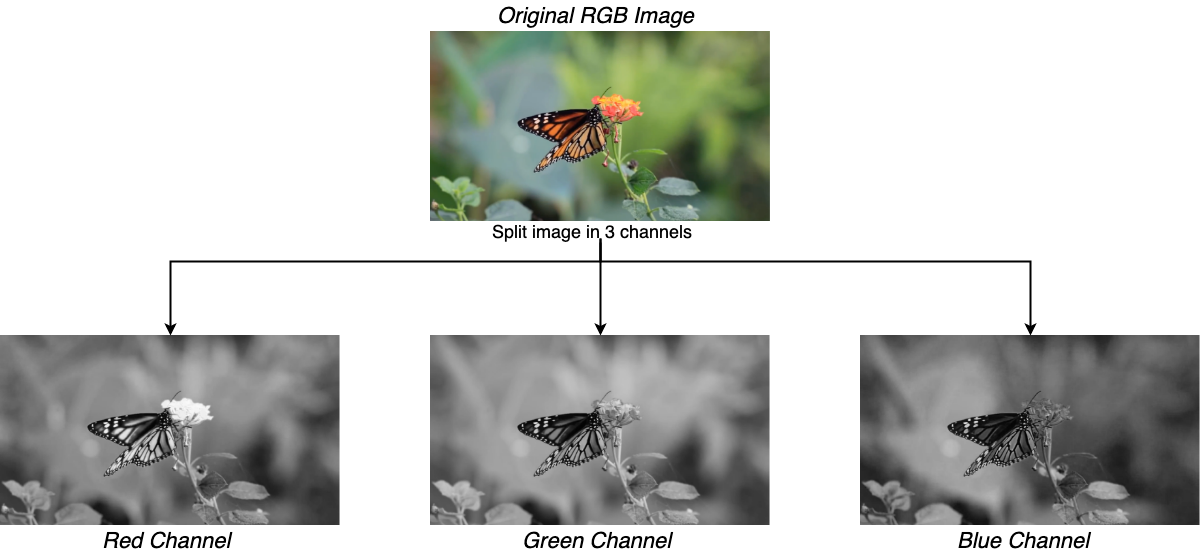
\includegraphics[width=\textwidth]{figures/implementation/rgb_image_channel_split.png}}
\caption{\label{fig:implementation-rgb_image_channel_split}The three colour channels that make up an coloured RGB image.}
\end{figure}

The RGB histogram is similar to the previously mentioned greyscale histograms, except that there are three separate histograms rather than a single one. There is 2D histogram for each colour channel (one in red, one in blue and one in green), where the brightness levels of each pixel are represented for each of those three colour channels. Each of the stills resulting from the split depicted in Figure \ref{fig:implementation-rgb_image_channel_split} will have their own histograms, which will form a complete RGB histogram when merged.\\

In contrast to the greyscale histograms, frames do not need to be converted to a different colour space when constructing RGB histograms as they are directly imported into three channels by OpenCV's \textit{cv2.VideoCapture()} function. In a similar fashion to the greyscale histograms, 256 bins are used for the RGB histograms, representing the potential values that each pixel can take for each colour channel. The RGB histogram is a combination of three 2D histograms, which are illustrated by Equation \ref{eq:rgb-histogram}, where $g_i\in [0, 255]$ and $N_g(i)$ represents the number of pixels that have an intensity equal to $g$ for the colour channel $i$. For example, $H_{i=2}(60)$ represents the number of pixels in the third channel of the image (blue channel) with an intensity value of 60.

\begin{equation}
\label{eq:rgb-histogram}
    \sum_{i=0}^{2} H_i(g)=N_g[i]
\end{equation}

To implement RGB histograms in the system, OpenCV's \textit{calcHist()} is once again used. In an identical manner to the greyscale histogram, the frame is passed to the function along with the colour channel \textit{[i]}, which are all placed inside a for-loop to generate a histogram for the three colour channels:

\mint[fontsize=\footnotesize]{python}|histogram = cv2.calcHist([frame], [i], None, [256], [0, 256])|

At this point, the three individual histograms that have been generated for the three colour channels are merged into a single plot to build the RGB histogram, as depicted in Figure \ref{fig:implementation-rgb_not_normalised}.

\begin{figure}[h] 
\centerline{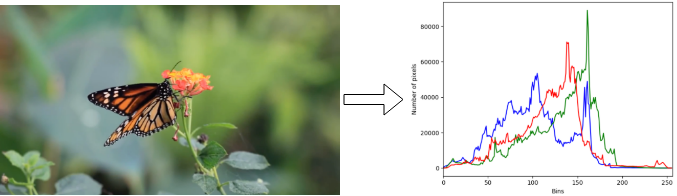
\includegraphics[width=\textwidth]{figures/implementation/rgb_not_normalised.png}}
\caption{\label{fig:implementation-rgb_not_normalised}The combination of the generated histograms for the three colour channels to construct the RGB histogram (not normalised).}
\end{figure}

Now that RGB histograms have been generated for each of the pre-selected frames (one frame every second), they are all stored in a dictionary made up of three keys, one for each colour channel. Each key links to a list where the histograms are stored away before being averaged into a single histogram used to create the second compact signature to represent the entire video. 

%%%%%%%%%%%%%%%%%%%%%%%%%%

\subsubsection{HSV Histogram Generation}

With the greyscale and RGB histograms now formed, the HSV histograms can finally be generated. HSV histograms make use of the HSV colour space, requiring the video frames to be converted from the original RGB colour space to the HSV colour space (see Figure \ref{fig:rgb_to_hsv}). The conversion is done using OpenCV's \textit{cv2.cvtColor()} function along with the \textit{cv2.COLOR\_BGR2HSV} attribute:

\mint[fontsize=\footnotesize]{python}|hsv_frame = cv2.cvtColor(frame, cv2.COLOR_BGR2HSV)|

\begin{figure}[h] 
\centerline{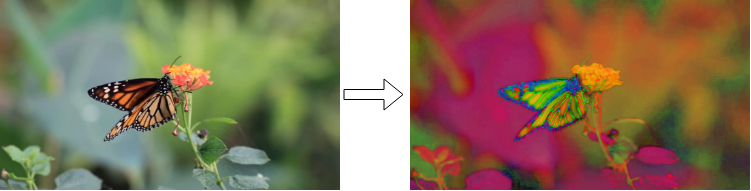
\includegraphics[width=\textwidth]{figures/implementation/rgb_to_hsv.png}}
\caption{\label{fig:rgb_to_hsv}Conversion of a frame from the RGB colour space to the HSV colour space.}
\end{figure}

This type of histogram is more complex to generate as it is not a 2D histogram like the previous greyscale and RGB histograms, but a 3D histogram. Because they are represented in 3D rather than 2D due to the particularities of the HSV colour space, less bins can be used to plot the data as pixels fall into bins when they are in conjunction with the range of the three channels (the pixels values must be within the range of the hue \underline{AND} the saturation \underline{AND} the value). Therefore, to avoid creating a histogram that is neither too coarse nor too sparse, 8 bins are used for the hue channel, 12 bins are used for the saturation channel, and 3 bins are used for the value channel, resulting in a histogram of 288 values\footnote{$8*12*3=288$}. This histogram is approximately the same length as the $256$ values previously used for the greyscale histograms and $3*256$ values for the RGB histograms. The histogram is described by Equation \ref{eq:hsv-histogram}, where $N(h,s,v)$ represents the number of pixels that fall within the range of the bin with values $h$ \underline{AND} $s$ \underline{AND} $v$.\\
\begin{equation}
\label{eq:hsv-histogram}
    H(h,s,v)=N(h,s,v)
\end{equation}

For example, a pixel with values $H(h=31, s=245, v=200)$ will fall into a bin with\footnote{Assuming ranges of 0-180 for Hue, 0-256 for Saturation, 0-256 for Value.}:
\begin{itemize}
    \item a hue value between 22.5 and 45 (bin \#2/8) \underline{AND}
    \item a saturation value between 234.6 and 256 (bin \#12/12) \underline{AND} 
    \item a value intensity between 170.7 and 256 (bin \#3/3).
\end{itemize}
The number of pixels in this bin will be $N(1,11,2)$ (0-based indexes).\\

Implementing the calculation of an HSV histogram in the system is again achieved through the use of OpenCV's \textit{calcHist()} function, with the result shown in Figure \ref{fig:implementation-hsv_not_normalised}. Similar arguments are passed such as the frame and an empty mask, but the arguments controlling the size of the histogram are different. In the code snippet below, \textit{[0, 1, 2]} indicates that the histogram has three channels (H, S and V), \textit{(8, 12, 3)} specifies the number of bins for each channel, and \textit{[0, 180, 0, 256, 0, 256]} marks the ranges of these bins:

\mint[fontsize=\footnotesize,breaklines]{python}|histogram = cv2.calcHist([hsv_frame], [0, 1, 2], None, (8, 12, 3), [0, 180, 0, 256, 0, 256])|

\begin{figure}[h] 
\centerline{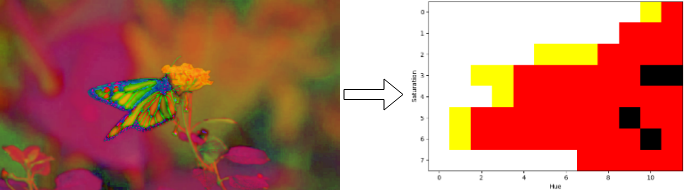
\includegraphics[width=\textwidth]{figures/implementation/hsv_not_normalised.png}}
\caption{\label{fig:implementation-hsv_not_normalised}The generated 3D HSV histogram (not normalised).}
\end{figure}

To conclude this offline colour-based extraction phase, HSV histograms are finally generated. Once all the HSV histograms are generated for each pre-selected frame, they are all stored in a list, like for the greyscale and RGB histograms. With the greyscale, RGB and HSV histograms all generated for each pre-selected frame of the video; these can now be averaged into a single compact signature for each histogram, which is explained in the next section.

%%%%%%%%%%%%%%%%%%%%%%%%%%%%%%%%%%%%%%%%%%%%%%%%%%%%%%%%%%%%%%%%%%%%

\subsection{Compact Video Signature}
\label{sec:implementation-compact-video-signature}

At this stage of the offline colour-based extraction phase, multiple greyscale, RGB and HSV histograms have been generated for each pre-selected frame for a video. Each of these histograms can now be averaged into one single histogram per colour model for each video. This means that each database video will be represented by one averaged greyscale histogram, one averaged RGB histogram and one averaged HSV histogram. This is achieved by looping through all the histograms' bins generated per video and calculating a new averaged value for each bin. For reminders, this process is repeated for every video in the database.\\

For the \textbf{greyscale histograms}, the 256 bins of the $N$ generated histograms are looped through and averaged (see Equation \ref{eq:average-greyscale-histogram}) to create a new mean value, where $H_n(i)$ corresponds to the number of pixels for the video's $n^{th}$ histogram at intensity $i$.
\begin{equation}
\label{eq:average-greyscale-histogram}
    \sum_{n=0}^{N} \frac{\sum_{i=0}^{255} H_n(i)}{N}
\end{equation}

The averaged value is then stored into the corresponding $i_{th}$ bin of the new histogram. For example, if $N=10$ (the video had ten pre-selected frames, so ten greyscale histograms were generated for that video), then for each of the 256 bins, the values of the ten histograms at that bin are averaged and the mean is stored in the new histogram.\\

Once all the bins have been averaged and added to the new histogram, that averaged histogram is normalised to obtain scale invariance between the histograms of the different videos. Instead of representing the number of pixels that fall into a bin, a normalised histogram represents a relative percentage count of the number of pixels in each bin, as depicted in Figure \ref{fig:implementation-normalise-histogram}. This is a necessary step in cases where the video frames have different sizes (the larger frames to have more pixels than the smaller frames) as the histograms can be more accurately compared when they represent a relative percentage rather than an integer count. The normalisation is achieved through OpenCV's \textit{cv2.normalize()} function:

\mint[fontsize=\footnotesize]{python}|histogram = cv2.normalize(histogram, histogram)|

\begin{figure}[h] 
\centerline{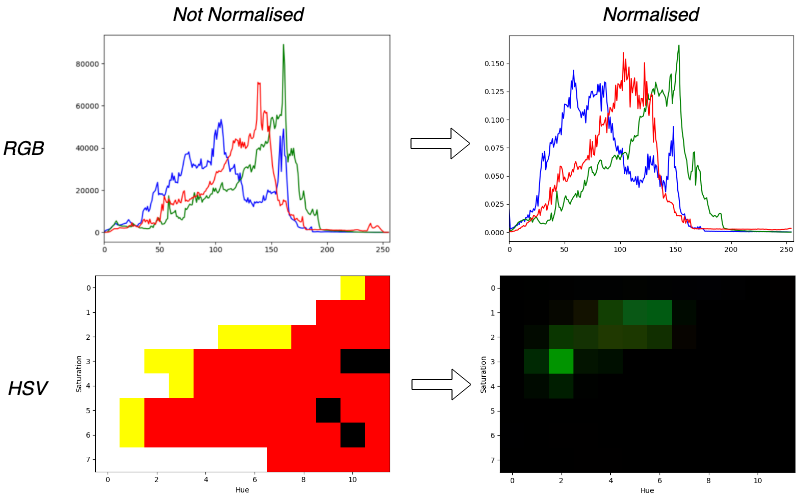
\includegraphics[width=0.85\textwidth]{figures/implementation/normalise-histogram.png}}
\caption{\label{fig:implementation-normalise-histogram}Normalising RGB and HSV histograms.}
\end{figure}

Finally, the averaged and normalised histogram values are stored in a plain text file as float values to maintain the precision, which is implemented using NumPy's \textit{np.savetxt()} function:

\mint[fontsize=\footnotesize,breaklines]{python}|np.savetxt("../histogram_data/{}/hist-{}".format(self.file_name, "gray"), avg_histogram, fmt='%f'))|

With the greyscale averaged and normalised histogram now stored in a plain text file, the same steps are repeated for the \textbf{RGB histogram} and \textbf{the HSV histogram}, with a few differences in the loops. First, for the RGB histograms, steps identical to the greyscale histogram's are followed for the three colour channels rather than a single time (see Equation \ref{eq:average-rgb-histogram}).

\begin{equation}
\label{eq:average-rgb-histogram}
    \sum_{h}^{(r,g,b)} (\sum_{n=0}^{N} \frac{\sum_{i=0}^{255} H_{h,n}(i)}{N_h})
\end{equation}

Second, for the HSV histograms, the histogram averaging is done by looping through each hue, saturation and value bin, since it is a 3D histogram and not a 2D histogram (see Equation \ref{eq:average-hsv-histogram}).

\begin{equation}
\label{eq:average-hsv-histogram}
    \sum_{n=0}^{N}(\sum_h \sum_s \sum_v H_n(h,s,v))
\end{equation}

Finally, the \textit{cv2.normalize()} and \textit{np.savetxt()} functions are used to normalise and save the average RGB and HSV histograms to plain text files. Samples of the saved plain text files for the butterfly video can be found in Appendix \ref{sec:appendix-txt-greyscale} for the greyscale histogram, in Appendix \ref{sec:appendix-txt-rgb} for the RGB histogram and in Appendix \ref{sec:appendix-txt-hsv} for the HSV histogram.\\

The final result of the offline colour-based feature extraction phase is a set of three averaged histograms that represent an entire video, with the values saved in three separate plain text files, as depicted in Figure \ref{fig:implementation-all_avg_norm_histograms}.\\

These histograms can be displayed using Matplotlib as they are being generated based on a flag passed on program start up. If the \textit{``--showhists''} flag is passed, then all averaged histograms are displayed before being saved in plain text files. As it takes approximately three seconds to process a single video in order to generate and store the three averaged histograms, the entire phase can take a while depending on the number of videos in the database. Therefore, a spinner is employed to indicate that the system is performing computations, which is implemented using Py-Spin\footnote{Py-Spin: \url{https://github.com/lord63/py-spin}}, a third-party library used to implement console-based spinners. The spinner, coupled with the histograms being displayed as they are being calculated, gives an visual indication that progress is being made.\\

With the colour-based features now saved in text files, they can be used multiple times in the online retrieval phase without needing to be re-generated, unless changes are made to the database videos, e.g. adding or removing videos.

\begin{figure}[h] 
\centerline{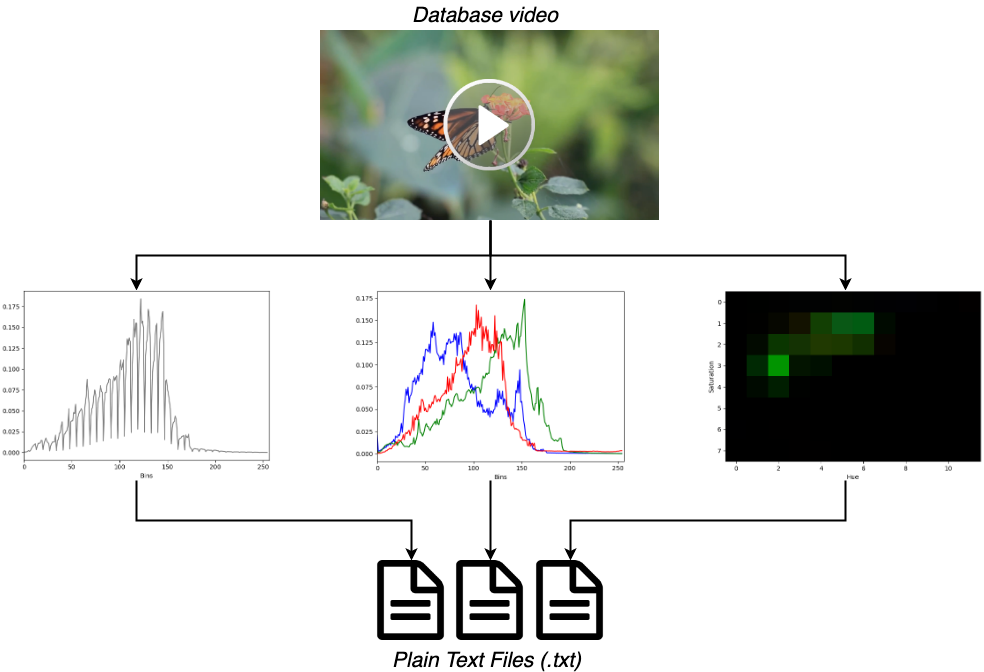
\includegraphics[width=\textwidth]{figures/implementation/all_avg_norm_histograms.png}}
\caption{\label{fig:implementation-all_avg_norm_histograms}The three average histograms generated for each database video and saved in plain text files.}
\end{figure}

%%%%%%%%%%%%%%%%%%%%%%%%%%%%%%%%%%%%%%%%%%%%%%%%%%%%%%%%%%%%%%%%%%%%
%%%%%%%%%%%%%%%%%%%%%%%%%%%%%%%%%%%%%%%%%%%%%%%%%%%%%%%%%%%%%%%%%%%%
%%%%%%%%%%%%%%%%%%%%%%%%%%%%%%%%%%%%%%%%%%%%%%%%%%%%%%%%%%%%%%%%%%%%

\section{Online Retrieval}

This section details the different steps that go towards matching a query video to one of the database videos using the colour-based features extracted in Section \ref{sec:implementation-offline-colour-based-feature-extraction}. The first step consists in processing the recorded query video to get rid of undesired artefacts such as poor framing (e.g. camera not properly positioned) and unwanted camera movements (e.g. shaky camera). Once the query is finished being processed, the same colour-based features previously extracted for all the database videos in the form of greyscale, RGB and HSV histograms are used to compute the similarities between the query video and each database video by measuring the distance between the histograms. The video with the highest score will be the match found by the system, which can be displayed to the screen to show the final result.

%%%%%%%%%%%%%%%%%%%%%%%%%%%%%%%%%%%%%%%%%%%%%%%%%%%%%%%%%%%%%%%%%%%%

\subsection{Query Video Pre-processing}

\subsubsection{Video Stabilisation}

The first improvement that can be made to the query is video stabilisation. Video stabilisation is implemented through the VidStab\footnote{Python Video Stabilisation: \url{https://github.com/AdamSpannbauer/python_video_stab}} third-party library, which is a quick solution to prune query videos with shaky movements. Additionally, an option to extend the query's borders to maintain the original frame size is available to prevent losing information.\\

The library is implemented in a custom class, which can be found in \ref{sec:code-stabilise-query-video}. A ``yes/no'' question is displayed on the console, giving a choice to stabilise the query video or not. If ``yes'' is chosen, the system first checks if a potential version of the video has already been previously stabilised and stabilises the query if it has not been stabilised already. Similarly to the previous phase, a spinner is used to indicate that the video is being stabilised as the process takes around twenty seconds for a ten second-long video. If ``no'' is chosen, then the system again checks for potential stabilised versions to use; otherwise, it uses the original version.

\subsubsection{Region of Interest Selection}

The second improvement that can be carried out to the query is selecting a Region Of Interest (ROI). Selecting an ROI involves cropping the query video to select only the area with the actual object of interest. In this case, this involves selecting the video playing on a display.\\

ROI selection is achieved through OpenCV's GUI functionality, which is employed through multiple functions such as a function to display images using \textit{cv2.imshow()}, draw on them using \textit{cv2.rectangle()}, and record mouse events by writing a callback function named \textit{click\_and\_crop()}:

\mint[fontsize=\footnotesize]{python}|cv2.setMouseCallback("Select ROI", self.click_and_crop)|

These three functionalities are combined in the system to display the first frame of the query video and allow a manual selection of two points on the frame. The first point is selected when the left mouse button is pressed using \textit{cv2.EVENT\_LBUTTONDOWN}, and the second point is selected when the button is unpressed using \textit{cv2.EVENT\_LBUTTONUP}. With these two points, a rectangle can be drawn on the frame to indicate the area that was selected. If the rectangle is correctly drawn, the \textit{`C'} key can be pressed to perform the cropping action; otherwise the \textit{`R'} key can be pressed to erase the rectangle and attempt to re-draw it until a satisfactory ROI is selected. The point coordinates are then used to ignore all the pixels outside the drawn rectangle when generating the compact histogram signatures of the query video, as sketched in Figure \ref{fig:implementation-roi_selection}. The full implementation of the code can be found in Appendix \ref{sec:code-roi-selection}.\\

\begin{figure}[h] 
\centerline{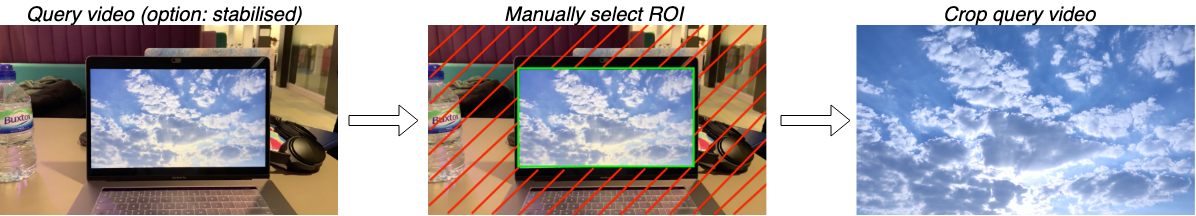
\includegraphics[width=\textwidth]{figures/implementation/roi_selection.png}}
\caption{\label{fig:implementation-roi_selection}The process of manually selecting a ROI to crop the query video.}
\end{figure}

Once the video query has been processed for stability and ROI selection, the same colour-based features from the offline extraction phase can be extracted before being compared to the database videos' features.

%%%%%%%%%%%%%%%%%%%%%%%%%%%%%%%%%%%%%%%%%%%%%%%%%%%%%%%%%%%%%%%%%%%%

\subsection{Matching Query to a Database Video}

\subsubsection{Query Video Feature Extraction}

In order to compare the query video to all the database videos, the same colour-based features described in Section \ref{sec:implementation-offline-colour-based-feature-extraction} need to be extracted first. A compact signature is generated for the query video in the form of an averaged greyscale histogram, an averaged RGB histogram and an averaged HSV histogram. The identical functions written for the offline colour-based feature extraction phase are re-used to generate the query video's histograms. This is achieved through a function parameter named \textit{is\_query}, which is a boolean that enters more sections of the function when it is true, such as selecting an ROI:

\mint[fontsize=\footnotesize]{python}|def generate_video_rgb_histogram(self, is_query=False, cur_ref_points=None):|

Once these histograms are generated, they can be compared to the histograms of each database videos.

\subsubsection{Distance Measurements}

At this stage of the pipeline, all of the database videos and the query video have now been analysed to create the compact signatures required to compute the similarities between the query video and the database videos. The similarity measurements are done by measuring the distance between each of the database videos' histograms with the query video's histograms. Four different distance metrics are used to compare the 2D greyscale and RGB histograms, while two distance metrics are used to calculate the similarities between the 3D HSV histograms.\\

The calculations between two 2D histograms are achieved through OpenCV's \textit{cv2.compareHist()} function, where the two histograms to compare are passed along with the method of choice:

\mint[fontsize=\footnotesize]{python}|comparison = cv2.compareHist(query_hist, rgb_video_hist, method)|

For the 3D HSV histograms, SciPy's statistical distances are used to calculate the distance between the different bins. The six different methods used are detailed below, where $d(H_1, H_2)$ represents the distance between a histogram $H_1$ and a histogram $H_2$, and $I$ represents the number of bins in the histograms.

\begin{enumerate}

    \item \underline{Correlation}:\\
    This is a metric that indicates the linear relationship between two histograms. The result of this metric ranges between $-1 < d(H_1,H_2) < 1$, where -1 represents a negative correlation, 0 an absence of correlation and 1 a high positive correlation. The closer the two histograms are to each other, the closer their correlation will be to 1. Equation \ref{eq:correlation} describes how this metric can be calculated.
    \begin{equation}
    \label{eq:correlation}
        d(H_1,H_2)=\frac{\sum _I(H_1(I)-\bar{H_1})(H_2(I)-\bar{H_2})}{\sqrt{\sum _I(H_1(I)-\bar{H_1})^2(H_2(I)-\bar{H_2})^2}}
    \end{equation}
    where $\bar{H_k}=\frac{1}{N}\sum_JH_k(J)$ and $N$ is equal to the total number of bins in the histogram. This metric is available through OpenCV's \textit{cv2.HISTCMP\_CORREL} attribute:
    \mint[fontsize=\footnotesize,breaklines]{python}|comparison = cv2.compareHist(query_hist['grey'], dbvideo_hist_grey, cv2.HISTCMP_CORREL)|
    
    \item \underline{Intersection}:\\
    This metric calculates the similarity between two histograms by superposing the two histograms and calculating how important the superposition is for each bin in the histogram. A value of 0 for a bin indicates that there is no overlap between the two histograms at that bin. The higher the intersection, the more the two histograms have in common, as portrayed by Equation \ref{eq:intersection}.
    \begin{equation}
    \label{eq:intersection}
        d(H_1,H_2)=\sum_Imin(H_1(I),H_2(I))
    \end{equation}
    Intersection is implemented through OpenCV's \textit{cv2.HISTCMP\_INTERSECT} attribute:
    \mint[fontsize=\footnotesize,breaklines]{python}|comparison = cv2.compareHist(query_hist['grey'], dbvideo_hist_grey, cv2.HISTCMP_INTERSECT)|
    
    \item \underline{Chi-Square Distance}:\\ 
    This metric uses the chi-square test $\chi^2=\frac{(a-b)^2}{a}$ in the form of a distance function described by Equation \ref{eq:chi-square}. The lower the value, the more the data from $H_1$ fits the data from $H_2$ and vice versa, the higher the value, the less the data from $H_1$ fits the data from $H_2$.
    \begin{equation}
    \label{eq:chi-square}
        d(H_1,H_2)=\sum_I\frac{(H_1(I)-H_2(I))^2}{H_1(I)}
    \end{equation}
    Therefore, the database video that will match the query the most is the one with the lowest chi-square distance. The chi-square distance is implemented in the code by using OpenCV's \textit{cv2.HISTCMP\_CHISQR}:
    \mint[fontsize=\footnotesize,breaklines]{python}|comparison = cv2.compareHist(query_hist['grey'], dbvideo_hist_grey, cv2.HISTCMP_CHISQR)|
    
    % \item \underline{Alternative Chi-Square}:\\
    % This metric uses an alternative to the first chi-square test $\chi^2=2\cdot \frac{(a-b)^2}{a+b}$ with the same properties (see Equation \ref{eq:alternative-chi-square}).
    % \begin{equation}
    % \label{eq:alternative-chi-square}
    %     d(H_1,H_2)=2\cdot \sum_I\frac{(H_1(I)-H_2(I))^2}{H_1(I)+H_2(I)}
    % \end{equation}
    % This alternative to the first chi-square distance is implemented in OpenCV by using \textit{cv2.HISTCMP\_CHISQR\_ALT}:
    % \mint[fontsize=\footnotesize,breaklines]{python}|comparison = cv2.compareHist(query_hist['grey'], dbvideo_hist_grey, cv2.HISTCMP_CHISQR_ALT)|
    
    \item \underline{Hellinger Distance} (using Bhattacharyya Coefficient):\\
    The Hellinger distance is used to quantify the difference between two discrete probability distributions (see Equation \ref{eq:hellinger}). The smaller the value, the closer the two histograms are to each other.
    \begin{equation}
    \label{eq:hellinger}
        d(H_1,H_2)=\sqrt{1-\frac{1}{\sqrt{\bar{H_1}\bar{H_2}N^2}}\sum_I\sqrt{H_1(I)\cdot H_2(I)}}
    \end{equation}
    where $\bar{H_k}=\frac{1}{N}\sum_JH_k(J)$ and $N$ is equal to the total number of bins in the histogram. The Hellinger metric is implemented in the code through OpenCV's \textit{cv2.HISTCMP\_HELLINGER} (although the OpenCV method is named Bhattacharyya, it actually uses the Hellinger distance but was named Bhattacharyya by the library developers because it uses the Bhattacharyya coefficient):
    \mint[fontsize=\footnotesize,breaklines]{python}|comparison = cv2.compareHist(query_hist['grey'], dbvideo_hist_grey, cv2.HISTCMP_HELLINGER)|
    
    % \item \underline{Kullback Leibler Divergence}:\\
    % The KL Divergence is normally used to calculate how much information is lost between two distributions 
    % \begin{equation}
    %     d_{KL}(H_1||H_2)=\sum_I H_1(I)\cdot log(\frac{H_1(I)}{H_2(I)})
    % \end{equation}
    
    \item \underline{Earth's Mover Distance} (Wassertein Distance):\\
    The Earth's Mover Distance, also known as Wassertein Distance, is a metric used to measure the dissimilarity between two distributions. The EMD depicted in Equation \ref{eq:emd} is calculated by measuring the least amount of moves required to transform one histogram into the other. Therefore, the smaller the EMD is, the more similar two histograms are to one another.
    \begin{equation}
    \label{eq:emd}
        EMD(H_1,H_2)=\sum_I |EMD_I(H_1,H_2)|
    \end{equation}
    where:
        \begin{itemize}
            \item $EMD_0 = 0$
            \item $EMD_{I+1}(H_1,H_2) = H_1(I)+EMD_I-H_2(I)$
        \end{itemize}
    The EMD between two histograms is implemented by looping through each slice of the 3D HSV histogram and using SciPy's \textit{scipy.stats.wasserstein\_distance()} function on each slice:
    
\begin{minted}[baselinestretch=0.9,bgcolor=LightGray,fontsize=\footnotesize,linenos,breaklines]{python}
comparison = 0
for h in range(0, self.bins[0]):  # loop through hue bins
    for s in range(0, self.bins[1]):  # loop through saturation bins
        comparison += wasserstein_distance(query_histogram['hsv'][h][s], dbvideo_hsv_histogram[h][s])
\end{minted}
        
    \item \underline{Energy Distance}:\\
    The Energy Distance is a metric used the cumulative distribution functions of two distributions to measure the distance between two histograms (see Equation \ref{eq:energy-distance}). The smaller the distance is, the closer the two histograms are, with $d(H_1,H_2)=0$ being identical histograms.
    \begin{equation}
    \label{eq:energy-distance}
        d(H_1,H_2) = \sqrt{2\mathbf{E}|X-Y|-\mathbf{E}|X-X'|-\mathbf{E}|Y-Y'|)}
    \end{equation}
    where: $X$ and $X'$ are independent random variables with the probability distribution $H_1$ and $Y$ and $Y'$ are independent random variables with the probability distribution $H_2$.  The Energy Distance between two histograms is implemented by looping through each slice of the 3D HSV histogram and using SciPy's \textit{scipy.stats.energy\_distance()} function on each slice:
    
\begin{minted}[baselinestretch=0.9,bgcolor=LightGray,fontsize=\footnotesize,linenos,breaklines]{python}
comparison = 0
for h in range(0, self.bins[0]):  # loop through hue bins
    for s in range(0, self.bins[1]):  # loop through saturation bins
        comparison += energy_distance(query_histogram['hsv'][h][s], dbvideo_hsv_histogram[h][s])
\end{minted}
    
\end{enumerate}

All of the distance metrics and histogram models are finally combined to produce the final result. For each histogram model distance metric used, scores indicating the similarities between each database video and the query video are calculated. A table is printed in the console to display the distance results for each metric and histogram model using the TerminalTables\footnote{TerminalTables: \url{https://github.com/Robpol86/terminaltables}} third-party library. An example of the printed console table using the library can be found in Appendix \ref{ch:appendix-raw-console-output-example}. Additionally, the data is also written to multiple CSV files to further analyse in specialised tools such as Excel and in order to read the output data of the online retrieval phase after the console has been cleared or closed.\\

Of all the scores calculated for each model and distance metric, the one revealing which database video matches the query the most is used to increment a dictionary. The increment relies on pre-defined weights assigned to each histogram model, which are detailed in Table \ref{tab:distance-metric-weights}:

\begin{itemize}
    \item \underline{Greyscale} histograms are the least descriptive model, with only one channel which cannot represent colours. The lowest weight worth one is therefore attributed to these.
    \item \underline{RGB} histograms use three channels and can describe the colours in a frame. They are therefore attributed a weight of 5.
    \item \underline{HSV} histograms are the most complex histograms employed in the system as they use three channels to describe how human vision perceives colours, plotting the results in 3D histograms. The highest weight worth ten is therefore attributed to these.
\end{itemize}

\begin{table}[h]
\centering
\resizebox{\textwidth}{!}{%
\begin{tabular}{|c|l|c|}
\hline
\textbf{Histogram Model} & \multicolumn{1}{c|}{\textbf{Distance Measurement}} & \textbf{Weight} \\ \hline
\multirow{4}{*}{\textbf{Greyscale}} & Correlation & 1 \\ \cline{2-3} 
 & Intersection & 1 \\ \cline{2-3} 
 & Chi-Square & 1 \\ \cline{2-3} 
 & Hellinger & 1 \\ \hline
\multirow{4}{*}{\textbf{RGB}} & Correlation & 5 \\ \cline{2-3} 
 & Intersection & 5 \\ \cline{2-3} 
 & Chi-Square & 5 \\ \cline{2-3} 
 & Hellinger & 5 \\ \hline
\multirow{2}{*}{\textbf{HSV}} & Wassertein distance (Earth's Mover Distance) & 10 \\ \cline{2-3} 
 & Energy Distance & 10 \\ \hline
\end{tabular}%
}
\caption{Weights used for the distances calculated based on the histogram model and the metric used. High importance is given to HSV results, medium importance to RGB results, and low importance to greyscale results.}
\label{tab:distance-metric-weights}
\end{table}

This dictionary is used at the end of the pipeline to determine which video was matched the most based on the number of occurrences in the dictionary. This number is converted into a probability of the videos in this dictionary to match the query video, which is plotted into a simple histogram using Matplotlib to visualise which video is matched the most, as shown in the left-hand side of Figure \ref{fig:implementation-online-retrieval-results}. The final result is displayed in the form of a figure that includes the first frames of the query video and the matched video, along with the runtime in seconds and the accuracy $Accuracy = \frac{True \quad Positives}{Number \quad of \quad Matches}$ of the match, which is depicted in the right-hand side of Figure \ref{fig:implementation-online-retrieval-results}.\\

\begin{figure}[h] 
\centerline{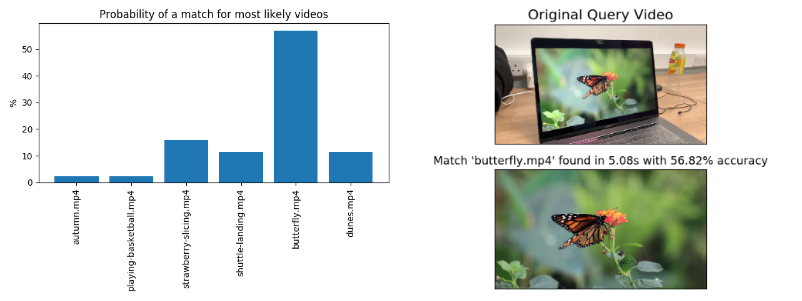
\includegraphics[width=\textwidth]{figures/implementation/online-retrieval-results.png}}
\caption{\label{fig:implementation-online-retrieval-results}Example of the results at the end of the online retrieval phase. In the left-hand side is a histogram showing the probability in percentage \% of the most likely videos to match the query. In the right-hand side is a figure presenting the final results, including the first frames of the query video and the match video along with the runtime and the accuracy of the match.}
\end{figure}

Once this figure with the final results is displayed, the program exits, marking the end of the pipeline. The online retrieval phase can be repeated any number of times using different query recordings of one of the database videos, without the need to run the offline colour-based extraction phase again.

%%%%%%%%%%%%%%%%%%%%%%%%%%%%%%%%%%%%%%%%%%%%%%%%%%%%%%%%%%%%%%%%%%%%
%%%%%%%%%%%%%%%%%%%%%%%%%%%%%%%%%%%%%%%%%%%%%%%%%%%%%%%%%%%%%%%%%%%%
%%%%%%%%%%%%%%%%%%%%%%%%%%%%%%%%%%%%%%%%%%%%%%%%%%%%%%%%%%%%%%%%%%%%

\section{Database Pre-Processing}
\label{sec:database-pre-processing}

This section details the steps that go towards processing the database of videos with a shot boundary detection algorithm in order to segment a long video, e.g. feature-length movies.\\

The RGB histograms of two consecutive frames are generated and compared using the Kullback Leibler Divergence metric for each colour channel in the histogram (see Equation \ref{eq:shot-boundary-detection}). If the sum of the three distances is greater than a global pre-defined threshold, then the two consecutive frames are different enough to be interpreted as a shot change, and the frame index is added to a list of detected shot boundaries. A global threshold of 10 is used to detect shot boundaries, which was determined by running the code multiple times to determine a value that detects most transitions. This is implemented in the code using the same techniques mentioned in the previous techniques, employing the \textit{cv2.calcHist()} function to generate the histograms for the three colour channels and \textit{cv2.compareHist()} to compare the RGB histograms. 

\begin{equation}
\label{eq:shot-boundary-detection}
\begin{aligned}
    detection \quad if \sum_{h}^{(r,g,b)}d(H_1,H_2) & > 10 \\
    \sum_{h}^{(r,g,b)} (\sum_I H_{1,h}(I)\cdot log(\frac{H_{1,h}(I)}{H_{2,h}(I)}) & > 10
\end{aligned}
\end{equation}

Once the video has been processed, all of the frames with a KL divergence superior to the threshold are marked as shot boundaries. The KL divergence between the consecutive frames from a test video with a hard cut transition \textit{(A)}, a dissolve transition \textit{(B)} and a fade to black transition \textit{(C-E)}, portrayed in Figure \ref{fig:shot_boundary_detection_frames}, are plotted using Matplotlib, with the results depicted in Figure \ref{fig:shot_boundary_detection_example}.\\

\begin{figure}[h] 
\centerline{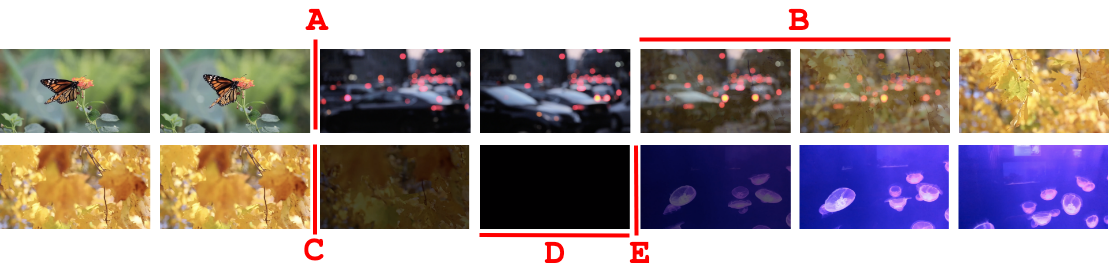
\includegraphics[width=\textwidth]{figures/implementation/shot_boundary_detection_frames.png}}
\caption{\label{fig:shot_boundary_detection_frames}Video frames used for the shot boundary detection algorithm.}
\end{figure}

\begin{figure}[h] 
\centerline{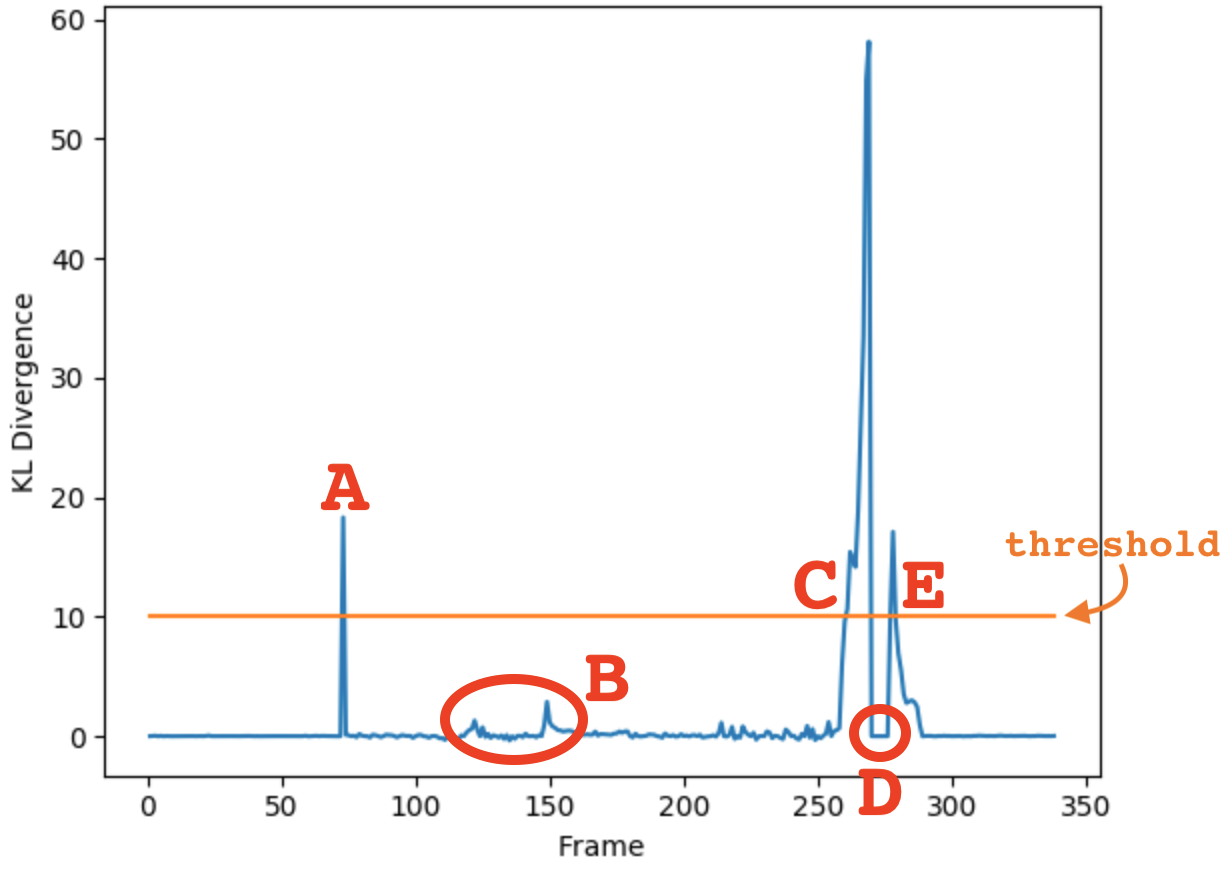
\includegraphics[width=0.70\textwidth]{figures/implementation/shot_boundary_detection_example.png}}
\caption{\label{fig:shot_boundary_detection_example}Example of the shot boundary detection algorithm on the test video from Figure \ref{fig:shot_boundary_detection_frames} using the Kullback Leibler Divergence to compare the RGB histograms between consecutive frames.}
\end{figure}

Using a global threshold approach to process consecutive frames detects hard cuts \textit{(A)} and fading to black cuts \textit{(C \& E)}, but does not detect a dissolve cut \textit{(B)} and detects the black frames in a fading to black transition as shot \textit{(D)}. However, this is a satisfying method to use for long videos as the goal is to extract a fraction of the frames rather than generate an exhaustive list of all the shots and scenes in a video. As mentioned earlier in Section \ref{sec:implementation-greyscale-histogram}, this algorithm is not included in the actual pipeline as short videos made of single shots and ranging from 7 to 14 seconds are used. However, it is used when testing with longer videos comprised of multiple shots.

%%%%%%%%%%%%%%%%%%%%%%%%%%%%%%%%%%%%%%%%%%%%%%%%%%%%%%%%%%%%%%%%%%%%
%%%%%%%%%%%%%%%%%%%%%%%%%%%%%%%%%%%%%%%%%%%%%%%%%%%%%%%%%%%%%%%%%%%%
%%%%%%%%%%%%%%%%%%%%%%%%%%%%%%%%%%%%%%%%%%%%%%%%%%%%%%%%%%%%%%%%%%%%

\section{Complete System Pipeline Flowchart}

Based on the detailed implementation of the system, a flowchart depicting the main aspects of the system can be found in Figure \ref{fig:CBVR-flowchart}.

\begin{figure}[h] 
\centerline{\includegraphics[width=1.20\textwidth]{figures/implementation/full-pipeline-flowchart.png}}
\caption{\label{fig:CBVR-flowchart}Complete flowchart of the system pipeline.}
\end{figure}

%%%%%%%%%%%%%%%%%%%%%%%%%%%%%%%%%%%%%%%%%%%%%%%%%%%%%%%%%%%%%%%%%%%%
%%%%%%%%%%%%%%%%%%%%%%%%%%%%%%%%%%%%%%%%%%%%%%%%%%%%%%%%%%%%%%%%%%%%
%%%%%%%%%%%%%%%%%%%%%%%%%%%%%%%%%%%%%%%%%%%%%%%%%%%%%%%%%%%%%%%%%%%%

\section{Code Structure}

This section covers the project structure of the implemented code, detailing what each directory and file represents. The entire code structure can be found online on GitHub: \url{https://github.com/Adamouization/Content-Based-Video-Retrieval-Code}.

\begin{itemize}
    \item \textit{``app''} directory: contains all the Python code used to implement the system.
    \begin{itemize}
        \item \textit{``main.py''} file: the starting point of the program. Parses command line arguments to determine whether to run in offline feature extraction phase, in online retrieval phase, or in database pre-processing phase.
        \item \textit{``histogram.py''} file: contains the \textit{HistogramGenerator} class with functions to generate, average, store and compare greyscale, RGB and HSV histograms.
        \item \textit{``video\_operations.py''} file: contains classes for video-related operations. The \textit{ClickAndDrop} class is used for manually selecting the Region of Interest and the \textit{VideoStabiliser} is used to stabilise the query video.
        \item \textit{``helpers.py''} file: contains multiple general-use functions such as retrieving file names, removing file extensions from filenames, displaying results in the form of plots or console outputs, parsing command line input and getting video information.
        \item \textit{``config.py''} file: contains global variables whose values are set by the command line arguments.
        \item \textit{``\_\_init\_\_.py''} file: default file required in any python package (cannot be deleted without causing errors).
    \end{itemize}
    \item \textit{``footage''} directory: where all the database of videos is located. A greyscale, RGB and HSV histogram is generated for each video in this directory. The query's histograms are then compared to each video's histograms from this directory.
    \item \textit{``histogram\_data''} directory: where the averaged greyscale, RGB and HSV histograms are stored as plain text files.
    \item \textit{``recordings''} directory: where all the pre-recorded query videos used to test the system are placed.
    \item \textit{``results''} directory: where general result-related files such as CSV and PNG files are placed.
    \item \textit{``requirements.txt''} file: the different technologies and third-party libraries required to run the code. The file is used by the Pip\footnote{PyPi: \url{https://pypi.org/}} system to install everything in a single installation.
    \item \textit{``README.md''} file: the instructions on how to setup and run the program locally.
\end{itemize}

%%%%%%%%%%%%%%%%%%%%%%%%%%%%%%%%%%%%%%%%%%%%%%%%%%%%%%%%%%%%%%%%%%%%
%%%%%%%%%%%%%%%%%%%%%%%%%%%%%%%%%%%%%%%%%%%%%%%%%%%%%%%%%%%%%%%%%%%%
%%%%%%%%%%%%%%%%%%%%%%%%%%%%%%%%%%%%%%%%%%%%%%%%%%%%%%%%%%%%%%%%%%%%

\section{Testing}

This project skips the implementation of a traditional testing suite with unit tests, integration tests and acceptance tests (Priority 3 Requirement F19). Rather than spending time writing an extensive testing suite, which is not very useful considering the nature of the project, the program is repetitively tested before committing changes to GitHub by using one of the database videos as the query video, which should always match that same video with 100\% accuracy (only true positives, no false positives).

%%%%%%%%%%%%%%%%%%%%%%%%%%%%%%%%%%%%%%%%%%%%%%%%%%%%%%%%%%%%%%%%%%%%
%%%%%%%%%%%%%%%%%%%%%%%%%%%%%%%%%%%%%%%%%%%%%%%%%%%%%%%%%%%%%%%%%%%%
%%%%%%%%%%%%%%%%%%%%%%%%%%%%%%%%%%%%%%%%%%%%%%%%%%%%%%%%%%%%%%%%%%%%

\section{Summary}

todo